\chapter{Treemap Evaluation for Software Evolution Data}
\label{ch:soft-eval}
\blfootnote{This chapter is based on the paper ``Quantitative Comparison of Dynamic Treemaps for Software Evolution Visualization'' \citep{vernier18software}}
% \title{Quantitative Comparison of Dynamic Treemaps for Software Evolution Visualization}

\textit{
As outlined in Chapter \ref{ch:intro}, one of our two research questions concerns how to extend treemapping algorithms to handle time-dependent hierarchical data. To do this, we need first and foremost to understand how existing treemapping algorithms fare when displaying dynamic data. In more detail, we also need to know how to quantitatively compare such algorithms. In this chapter, we address the above two questions by a first evaluation. For this, we consider a smaller scope in terms of datasets, focusing on dynamic hierarchies coming from evolving software repositories. Using this limited scope of datasets, and beyond evaluating existing treemapping algorithms, we introduce a stability metric for gauging the performance of such algorithms in the presence of time-dependent data, that quantifies the relationship between data change and change in the data's visualization using treemaps. We next extend this approach in Chapter \ref{ch:tree-eval} to reliably and fairly test treemapping algorithms on generalized data, \emph{i.e.}, a large number of datasets from different sources, displaying a variety of traits and dynamics, beyond dynamic hierarchies coming from software evolution.}


\vspace{5mm} %5mm vertical space

\noindent \textbf{Abstract:}
Dynamic treemaps are one of the methods of choice for displaying large hierarchies that change over time, such as those encoding the structure of evolving software systems. While quality criteria (and algorithms that optimize for them) are known for static trees, far less has been studied for treemapping dynamic trees. We address this gap by proposing a methodology and associated quality metrics to measure the quality of dynamic treemaps for the specific use-case and context of software evolution visualization. We apply our methodology on a benchmark containing a wide range of real-world software repositories and 12 well-known treemap algorithms. Based on our findings, we discuss the observed advantages and limitations of various treemapping algorithms for visualizing software structure evolution, and propose ways for users to choose the most suitable treemap algorithm based on the targeted criteria of interest.

\section{Introduction}
\label{sec:treemap_eval_intro}
%
Hierarchies play a central role in understanding large software systems. Such systems evolve over hundreds of revisions or more, and can have thousands of elements or more, which are typically organized hierarchically (\emph{e.g.} in folders, files, classes, and methods). Hence, tools for visually understanding evolving hierarchies are a key component in the program comprehension arsenal. Treemaps are a well known method for visualizing hierarchical data. Given an input tree whose leafs have several attributes, treemaps recursively partition a 2D spatial region into cells whose area, color, shading, or labels encode the tree's data attributes. Compared to other methods such as node-link~\citep{harel,frick} or Sunburst~\citep{sunburst,sunburst2} techniques, treemaps use all available screen pixels to show data and thus can handle trees of tens of thousands of nodes.

\emph{Dynamic} treemaps leverage the above advantages to show dynamic, or evolving, trees. Given a tree sequence, they create an animated sequence of treemap layouts that reflect how the structure and attributes of the trees in the sequence change in time. Evolving treemaps have been created both by using classical static treemap algorithms~\citep{treevis} or by specialized algorithms~\citep{sondag17,hees17,hahn10}.

Evolving treemaps have received great interest in software visualization\,\citep{diehl08,hees17,hahn10,fisher10,gotz11}. As many treemap techniques exist, the question emerged of how to measure their quality. For common rectangular treemaps, which map tree nodes to rectangles, visual quality is typically measured by the aspect ratio of these rectangles. However, the aspect ratio may not capture all desirable qualities of such treemaps. For example, bad aspect-ratio cells of a tiny area could influence the overall visual quality far less than large bad aspect-ratio cells. Atop visual quality, evolving treemaps are assessed by measuring their rate of visual change. However, this metric may not capture all desirable properties: Large visual changes in a treemap are expected (and actually desirable) when the underlying tree changes drastically, but undesired when the tree changes only slightly.

Although treemaps are used for over two decades in software visualization~\citep{shneiderman92,schulz11_treesurvey,treevis,landesberger11}, there are few comprehensive evaluations of the quality of dynamic treemap techniques and, to our knowledge, none that focuses on trees capturing software evolution. The aim of this chapter is to fill this gap. For this, we first review the related work in (dynamic) treemaps and their quality measurement, with a focus on software visualization (Sec.~\ref{sec:init-background}). We next refine desirable treemap properties into 5 quality metrics that capture both spatial quality and dynamic quality (Sec.~\ref{sec:init_metrics}). We measure these metrics on 12 well-known treemap algorithms on 28 tree sequences, ranging from a few hundred to tens of thousands of elements, all extracted from software repositories. We next visualize and analyze our results to address questions that practitioners would like to answer to choose a suitable technique (Sec.~\ref{sec:mat_aggr}). We discuss our findings and proposed methodology in Sec.~\ref{sec:init-discussion}. Our results (datasets, metrics, treemap implementations, evaluation results, and visualizations thereof) are publicly accessible for researchers in the software visualization field interested in evaluating treemap methods for evolving software hierarchies.

\section{Background}
\label{sec:init-background}
%
%
Hierarchies are arguably the central element in most software visualizations. They capture the physical (\emph{e.g.} files and folders) or logical software (\emph{e.g.} syntax tree) system structure, together with static or dynamic attributes, \emph{e.g.}, code size, quality metrics~\citep{lanza06}, change requests, or testing results~\citep{diehl08}. Both static and dynamic hierarchies in program comprehension are typically extracted by mining software repositories~\citep{lanza03,kagdi07}.
When small (a few hundred nodes), such trees can be visualized using classical node-link layouts such as in class or architecture diagrams~\citep{muller88,lanza03,telea02}. This works well for architecture-level views on a software system. However, code-level views, which contain nodes from subsystems all the way to classes and methods, generate large trees, having hundreds of thousands of nodes\,\citep{sunburst2}. These require space-filling methods, such as icicle plots~\citep{holten06,cornelissen07} or, the method of choice, treemaps. The latter are discussed below.

\subsection{Treemap algorithms}
%
%
Let $T=\{n_i\}$ be a tree with nodes $n_i$, and let $a_i \in \mathbb{R}^{+}$ be an attribute defined on the tree leaves. For non-leaf nodes $n_i$, $a_i$ equals the sum of the attributes of the children of $n_i$. A rectangular treemap algorithm $TM$ creates a set of rectangle cells $\{c_i\} = TM(T)$, $c_i \subset \mathbb{R}^2$ for the nodes $n_i$ so that the area of $c_i$ equals $a_i$ and children node cells create a partition of their parent cell. Several treemap algorithms exist, as follows (for detailed surveys, see\,\cite{schulz11_treesurvey,hci_treemaps,treevis,landesberger11}). Slice and dice (SND) treemaps pioneered the concept but were found to create too long-and-thin cells which are hard to grasp\,\citep{shneiderman92}. Subsequent algorithms tried to improve this aspect, quantified by the aspect ratio (AR) of the treemap cells. Squarified treemaps (SQR) propose a slicing heuristic that achieves, in general, very good (close to one) AR values~\citep{sqr}. Nagamochi and Abe refined this idea in an algorithm (APP) that approximates the optimal AR a given treemap can reach~\citep{nagamochi07}. However, SQR is not particularly \emph{stable} -- small changes in the input tree can yield large changes in the treemap layout. Several algorithms have aimed to improve stability. Ordered treemaps (OT)~\citep{ordered} and Strip treemaps (STR)~\citep{bederson02} lay out cells $c_i$ to follow a predefined order of the nodes $n_i$. Different algorithms propose different orderings: Pivot-by-Middle (PBM), Pivot-by-Size (PBZ), and Pivot-By-Split-Size (PBS)~\citep{ordered}; Engdahl's Split algorithm~\citep{engdahl}; and laying out cells along a space-filling curve, \emph{e.g.}, Spiral (SPI)~\citep{spiral}, and Hilbert (HIL) and Moore (MOO) fractal curves~\citep{hilbert_moore}. Spatially-Ordered Treemaps (SOT)~\citep{sot} extend SQR by ordering sibling nodes so that the most similar ones are processed in turn. NMap~\citep{nmap} uses a related idea; cells are placed according to the similarity of their attributes, using a dimensionality-reduction approach. Two versions exist: NMap Alternate Cuts (NAC) alternate horizontal and vertical cuts to subdivide the space (akin to SND), while NMap Equal Weights (NEW) splits the space to create similar-size cells. However, NMap was only applied to single-level trees. Recently, Sondag \emph{et al.} proposed stable treemaps~\citep{sondag17}, which aim to improve both the AR and stability for dynamic treemaps by using non-sliceable layouts.

Other cell shapes can be used besides rectangles. Voronoi treemaps~\citep{balzer05,balzer05b} exploit the properties of weighted Voronoi diagrams to create organic-looking visualizations where cells are convex polygons with, in general, good AR values. Voronoi methods have also been used, with good results, to construct dynamic treemaps for visualizing software structure evolution~\citep{hees17,gotz11}. Hybrid treemaps (HTM)~\citep{htm} combine various basic treemap techniques to generate the final layout. Other variants include jigsaw treemaps~\citep{jigsaw}, orthoconvex treemaps~\citep{deberg14}, and bubble treemaps~\citep{bubble}.

\subsection{Treemap quality metrics}
\label{sec:quality}
%
%
In practice, the quality of treemaps is measured using two types of metrics, as follows.

\noindent\emph{Spatial quality} metrics capture how easy one can read the information shown in a static treemap. Such metrics include the aspect ratio (AR) of the treemap cells, which ideally should equal one. For ordered treemaps, the readability metric measures how often one switches visual scanning direction while reading the treemap in order~\citep{bederson02}; and the continuity metric measures how often cells for neighbor nodes (following the given node order) are not neighbors in the treemap layout~\citep{spiral}.\\

\noindent\emph{Stability} metrics capture how easy one can follow the changes in a dynamic treemap. Given two  treemaps for two (typically consecutive) time-moments $t_i$ and $t_j$, \cite{ordered} define stability as the distance between the vectors $(x_k(t_i), y_k(t_i), w_k(t_i), h_k(t_i))$ and $(x_k(t_j), y_k(t_j), w_k(t_j), h_k(t_j))$, where $x$ and $y$ are the coordinates of the top-left corner, and $w$ and $h$, the width, and the height of a cell $c_k$, averaged over all cells in the treemap.
\cite{hahn10} use for stability the change of distance between the centroids of $c_k(t_i)$ and $c_k(t_j)$, averaged over all cells.
\cite{hilbert_moore} use the same cell-change metric (top-left corner, width, height) as \cite{ordered}, but aggregate via variance rather than average. They also propose a drift metric which measures how much a cell moves away from its average position over a time period. Two recent metrics measure stability at the level of pairs of cells rather than individual cells. \cite{Hahn2017} propose the relative direction change, which measures the angle change of centroids for every pair of cells in a layout. \cite{sondag17} measure the relative position change of each cell with respect to eight planar zones defined by four lines given by the edges of that cell, averaged over all treemap cells.

%ALEX: I didn't cite our EuroVis poster here since it doesn't introduce any new metrics as such

\subsection{Software visualization challenges}
\label{sec:current_state}
%
%
Summarizing, considerable effort went into designing static treemap methods and measuring their quality. Less effort went to evaluating dynamic treemaps. We identify limitations in several directions, with a focus on our use-case of visualizing large evolving software hierarchies:\\

\noindent\textbf{Algorithms:} Treemap papers typically compare a few (2--5) algorithms from the much larger set of available ones. In particular, it is not clear how most existing static treemap algorithms perform on the types of dynamic trees extracted from software evolution analyses.\\

\noindent\textbf{Datasets:} Existing methods are typically evaluated on one or a few datasets. While in this chapter, we cannot (and do not aim to) cover the full space of all possible trees, we can do better than existing work: For our specific context of software visualization, we aim to know how treemap methods perform on a representative collection of software hierarchies capturing software evolution.\\

\noindent\textbf{Metrics:} As outlined in Sec.~\ref{sec:quality}, stability is currently measured by looking at how much two treemaps (typically for consecutive time moments) change with respect to each other. However, when the underlying tree sequence changes a lot, \emph{e.g.} by insertions or deletions of many files or classes at the same moment during a software repository's evolution (an event well-known to take place often in software evolution), the treemap will change a lot, so its evolution will be labeled as unstable. However, it is actually \emph{desirable} to have a large visual change in this case, as this correctly shows the presence of a large data change. We argue that ways to measure stability as a function of the data change are needed.\\

\noindent\textbf{Result exploration:} Most evaluations consider only aggregated metrics with one value per technique or per technique-and-dataset. Analyzing the actual distribution of metric values over both layout-space and time can give extra insights into the strengths and weaknesses of specific techniques.\\

\noindent\textbf{Replicability:} Treemap evaluations can be hard to replicate as datasets and algorithm implementations are not always openly available or not integrated to make a comparison on different datasets, and along different metrics, easy. Replicability is a growing concern in information visualization but with particular weight in software visualization\,\citep{sensalire09,seriai14,merino18}.

The remainder of this chapter is dedicated to addressing the above points.


\begin{table}[htbp!]
\small
\centering
\scalebox{0.9}{
\begin{tabular}{|l|l|r|r|}
\hline
\textbf{Dataset} & \textbf{Revisions} & \textbf{Nodes (total)} & \textbf{Average depth} \\
\hline
animate.css & 50 & 3454 & 2.87\\
AudioKit & 22 & 11178 & 6.95\\
bdb & 62 & 2658  & 3.83\\
beets & 106   & 9844 & 3.75\\
brackets &  88  & 120292 & 12.85\\
caffe & 44 & 12969   & 4.93\\
calcuta & 50 & 2882 & 10.76\\
cpython   & 321 & 584821 & 6.50\\
earthdata-search   &  46& 18539 & 6.82\\
emcee & 64 & 1746  & 3.62\\
exo & 97 &  36436  & 11.88\\
fsharp   & 69 & 22906 & 7.89\\
gimp   & 72 &  170418 & 5.19\\
hospitalrun-frontend   & 38 &  16759 & 5.71\\
Hystrix & 61 & 15530  & 13.29\\
iina & 74 &  6849  & 4\\
jenkins & 137  & 277185 & 11.94 \\
Leaflet &  84  & 13381 & 4.86 \\
OptiKey   & 36 & 9782 & 6.72\\
osquery  & 37 & 14111 & 5.75 \\
PhysicsJS   & 20 & 2022 & 4.6\\
pybuilder   & 53 & 5457 & 7\\
scikitlearn   & 88 & 48468 & 5.75\\
shellcheck   & 53 & 746 & 2.39\\
soundnode-app   & 35 & 3196 & 6.88\\
spacemacs   & 51 & 10201 & 4.96\\
standard   & 29 & 203 & 2\\
uws & 122 & 4093 & 2.76\\
\hline
\hline
\textbf{Totals:} & 2132 & 1458036 & 5.77\\
\hline
\end{tabular}
}
\caption{Software evolution tree datasets used in the evaluation.}
\vspace{-0.2cm}
\label{tab:software_datasets}
\end{table}

\begin{figure*}[htbp!]
\centering
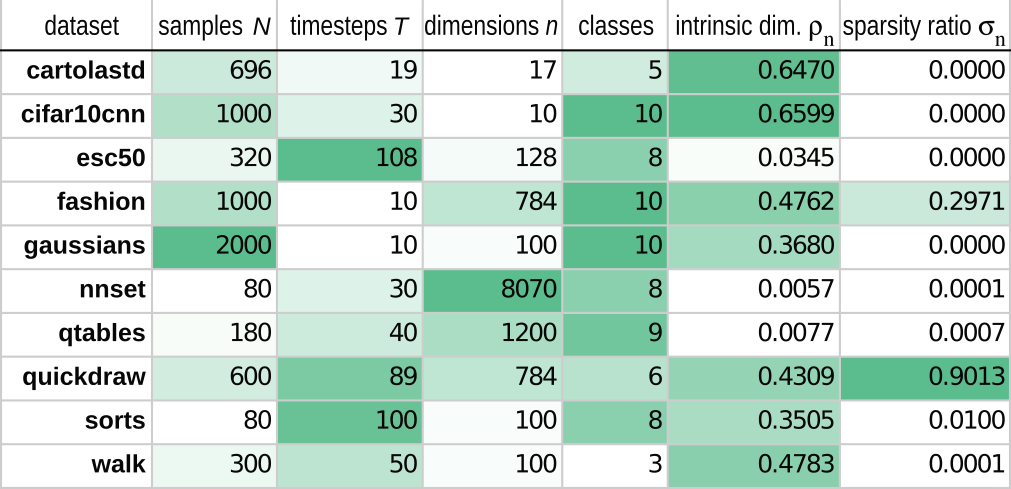
\includegraphics[width=\textwidth]{figures/initial-treemap-evaluation/datasets.eps}
\caption{Union trees of software evolution tree datasets used in the evaluation. Names correspond to public repositories on GitHub.}
\label{fig:datasets}
\end{figure*}


\section{Measuring the quality of dynamic treemaps}
\label{sec:init_metrics}
%
%
To address the current limitations of dynamic treemap evaluations in software visualization, we performed an in-depth study covering the five directions in Sec.~\ref{sec:current_state}, as follows.

\subsection{Algorithms}
\label{sec:mat_algos}
%
We consider in our evaluation 12 methods: Approximate (APP), Hilbert (HIL), Moore (MOO), NMap-Alternate-Cuts (NAC), NMap-Equal-Weights (NEW), Pivot-by-Middle (PBM), Pivot-by-Size (PBZ), Pivot-by-Split-Size (PBS), Slice-and-Dice (SND), Spiral (SPI), Squarified (SQR), and Strip (STR) treemaps. For NMap, we use as seed layout the one computed by SQR (for details, see\,\cite{nmap}). We do not consider non-rectangular treemap methods, as their quality is less easy to compare with rectangular ones, and are also less used in practice. Also, we do not consider the stable treemaps in~\citep{sondag17} as this method is considerably slower (over one order of magnitude) than the above-mentioned methods.

\subsection{Datasets}
\label{sec:mat_data}
%
We evaluate all above treemap methods on a collection of 28 datasets (Tab.~\ref{tab:software_datasets}). All of them consist of trees describing the hierarchy of public and well-known GitHub software repositories (folders, files, classes), one tree per revision, where leaves (classes) are attributed by their number of lines of code. The trees and their attributes have been extracted from the actual repositories by a fully automatic pipeline we built using \emph{libgit2}\,\citep{libgit2} for repository parsing and Understand\,\citep{understand} for code analysis. For a more detailed description of the extraction pipeline, we refer to~\cite{vmv}. The respective software projects have widely different sizes, tree depths and structures, durations, numbers of contributors, language (C, C++, Java, Python), and code type (library, framework, application). This is seen in the figures in Tab.~\ref{tab:software_datasets} and also in Fig.~\ref{fig:datasets} which shows the union trees $\cup_{i} T(t_i)$ for the considered datasets. Hence, we argue that this collection covers reasonably well the space of tree sequences obtained from software evolution.

\subsection{Metrics}
\label{sec:mat_metrics}
%
Let $w_k$ and $h_k$ be the width and height of cell $c_k$; and $(W,H)$ the width and height of the screen space we draw the treemap in. With these, we consider the following metrics.

\subsubsection{Spatial quality metric}
\label{sec:mat_met_spatial}
%
We first consider the classical aspect-ratio metric
%
\begin{equation}
Q^{AR}_k = \min(w_k,h_k)/\max(w_k,h_k).
\label{eqn:spatial_ratio}
\end{equation}
%
Introduced in~\cite{sqr}, this metric has been since then used by all treemap evaluations to capture spatial quality. As such, we keep it in our evaluation. It is designed to give high scores for rectangles with sides of similar length, and low scores otherwise.
%

\subsubsection{Stability metrics}
\label{sec:mat_met_stab}
%
Let $c_k(t_i)$ and $c_k(t_j)$ be two cells in two consecutive versions $T(t_i)$ and $T(t_j=t_{i+1})$ for the same node in a dynamic tree. Typical stability metrics (Sec.~\ref{sec:quality}) only measure the \emph{visual} change $\delta c_k$ between $c_k(t_i)$ and $c_k(t_j)$. We use for $\delta c_k$ the average sum of distances between the four corresponding corners of $c_k(t_i)$ and $c_k(t_j)$~\citep{ordered}, normalized by the treemap diagonal $\sqrt{W^2+H^2}$, so $\delta \in [0,1]$. We next define the \emph{data change} between nodes $n_k(t_i)$ and $n_k(t_j)$ as $\delta a_k = |a_k(t_i)-a_k(t_j)|$, where $a_k$ is the relative weight of $n_k$ at time $t_i$. If either of $n_k(t_i)$ or $n_k(t_j)$ does not exist, \emph{i.e.}, a node was created or deleted in versions $t_i$ or $t_j$, we set the respective $a_k$ to zero, which is as if the respective node was depicted by a zero-size cell. We normalize $a_k(t_i)$ by the weight sum of all nodes $n_k$ present at time $t_i$, so $\delta a_k \in [0,1]$. With this, we define the stability of a cell $c_k$ in a treemap in several ways. First, we define stability as
%
\begin{equation}
Q^{RATIO}_k =  (1-\delta c_k) / (1 - \delta a_k).
\label{eqn:stab_ratio_1}
\end{equation}
%
When visual changes are proportional to data changes, since both are normalized, $Q^{RATIO}_k$ goes to one. Note that an analogy to Eqn.~\ref{eqn:spatial_ratio}, \emph{i.e.}, $Q^{RATIO}_k=\min(\delta c_k, \delta a_k)/\max(\delta c_k, \delta a_k)$ does not work: Eqn.~\ref{eqn:spatial_ratio} is symmetric in width and height. For stability (Eqn.~\ref{eqn:stab_ratio_1}), we want to assess visual change as a function of data change, and not conversely.

\noindent A second way to define stability is by
%
\begin{equation}
Q^{MOD}_k = 1 - | \delta c_k - \delta a_k |.
\end{equation}
%
For proportional visual \emph{vs} data changes, $Q^{MOD}_k=1$.

\begin{figure}[htbp!]
\centering
\includegraphics[width=.6\textwidth]{figures/initial-treemap-evaluation/unavoidable.eps}
%\includegraphics[width=1.0\linewidth]{figures/unavoidable.eps}
\vspace{-0.1cm}
\caption{Computation of unavoidable change metric $Q^{UNAV}_k$.}
\vspace{-0.2cm}
\label{fig:unavoidable}
\end{figure}


%\noindent We compute ($Q_k^{RATIO}$ and $Q_k^{MOD}$) and area-weighted ($Q_k^{WRATIO}$ and $Q_k^{WMOD}$) versions of the above metrics, like in Eqn.~\ref{eqn:spatial_weighted}. For a whole tree, we average per-cell metrics, like for spatial metrics (Sec.~\ref{sec:mat_met_spatial}). }

To compare data and visual changes, $Q_k^{RATIO}$ and $Q_k^{MOD}$ must be normalized to the same range, therefore we clip $Q_k^{RATIO}$ to the $[0,1]$ interval. However, this can introduce normalization biases, \emph{e.g.} when the data changes and visual changes have very different ranges. To address this, we next propose to define stability purely in visual space. For this, we consider the actual change $\delta c_k$ of a cell \emph{vs} the \emph{unavoidable}, \emph{i.e.} minimal, change $\Delta c_k$ that $c_k$ would need to undergo to accommodate the data change from $a_k(t)$ to $a_k(t+1)$. If $\delta c_k > \Delta c_k$, the algorithm is unstable; if $\delta c_k = \Delta c_k$, it is fully stable. We compute $\Delta c_k$ as follows (Fig.~\ref{fig:unavoidable}). Let $c_k(t)$ be a cell of width $w$ and height $h$ at time step $t$. Let $c_k(t+1)$ be the version of $c_k(t)$, of area $a_k(t+1)$, at step $t+1$. We first note that $\delta c_k$ is minimal when $c_k(t)$ and $c_k(t+1)$ have the same center, as visual change is then caused \emph{purely} by data change and not by avoidable `drift' of the cell corners. Taking a $xy$ coordinate frame centered in this common cell center, the top-right corner of $c_k(t)$ is constrained to a hyperbola $y = a_k(t+1)/4x$. Hence the minimal change $\Delta c_k$ is four times the minimal distance $D$ from this corner to the hyperbola, \emph{i.e.}
%
\begin{equation}
D(x) = \sqrt{(x - w/2)^2 + (a_k(t+1)/4x - h/2)^2}. \nonumber
\end{equation}
%
To find the minimum of $D$, we solve $\frac{d D^2}{d x}=0$ for $x \geq 0$. This quartic equation in $x$ has analytic solutions. We obtain $x$, the width of the optimal cell $c_k(t+1)$, and thereby the minimal $\Delta c_k$. We define the unavoidable-motion stability as
%
\begin{equation}
Q^{UNAV}_k = 1 - (\delta c_k - \Delta c_k).
\end{equation}
%

Finally, we define stability for a whole tree $T$ as the \emph{absolute} value of the Pearson correlation coefficient
%
\begin{equation}
Q^{CORR} = \left| \frac{  \sum_k (\delta c_k - \overline{\delta c_k}) (\delta a_k - \overline{\delta a_k})  } {\sqrt { \sum_k (\delta c_k - \overline{\delta c_k})^2} \sqrt { \sum_k (\delta a_k - \overline{\delta a_k})^2}   }\right|
\label{eqn:pearson}
\end{equation}
%
of the signals $\{\delta c_k\}$ and $\{\delta a_k\}$ for all cells $c_k \in T$, where $\overline{\delta c_k}$ and $\overline{\delta a_k}$ are the signals' averages, so $Q^{CORR} \in [0,1]$. If visual and data changes $\delta c_k$ and $\delta a_k$ are linearly correlated, $Q^{CORR}$ reaches one. $Q^{CORR}$ close to zero indicates uncorrelated changes, \emph{i.e.}, instability.

\noindent Compared to existing treemap stability metrics~\citep{ordered,hahn10,hilbert_moore,sondag17}, all our above metrics consider the \emph{relation} of visual change $\delta c_k$ to data change $\delta a_k$. This is a fundamental difference: A treemap method $TM(T) = \{c_i\}$ is a \emph{function} from trees $T$ to cell-sets $\{c_i\}$, so its stability should be defined akin to Cauchy or Lipschitz continuity, which relate function-value ($\{c_i\}$) changes to variable ($T$) changes rather than measuring function changes only. Indeed: If a function's output strongly changes, the function \emph{itself} is not necessarily unstable; this can happen when the input variable strongly changes.

\subsubsection{Metric weighting}
%
As mentioned in Sec.~\ref{sec:treemap_eval_intro}, very small but bad aspect-ratio cells may not strongly influence the overall perceived spatial quality of a treemap, since they are barely visible. The same argument could be made for very small unstable cells \emph{vs} the overall perceived stability. To model these, when computing the average value of the metrics $Q^{AR}$, $Q^{RATIO}$, $Q^{MOD}$, and $Q^{UNAV}$, we weigh the respective per-cell values $Q^{AR}_k$ (and the other three ones) by the sizes $a_k$ of their cells. We used such weighted metrics in all experiments described next in Secs.~\ref{sec:q2}-\ref{sec:q4}. However, the obtained results showed that the aggregated weighted metric values differ only very slightly from their unweighted versions. As such, in the following we will only consider the unweighted metric versions.


\section{Result exploration}
\label{sec:mat_aggr}
%
We measure the five metrics (Eqns.~\ref{eqn:stab_ratio_1}-\ref{eqn:pearson}) on all 28 test datasets (Sec.~\ref{sec:mat_data}) processed by all 12 treemap methods (Sec.~\ref{sec:mat_algos}). We record metrics at the \emph{cell} level (except $Q^{CORR}$, recorded at tree level). This yields a high-dimensional-and-hierarchical dataset, conceptually a
 table with seven columns (5 metrics, algorithm ID, dataset ID, time step) and as many rows as the number of measured cells in all datasets, all timesteps. Exploring this data space is a challenge in itself. As noted in Sec.~\ref{sec:current_state}, current treemap evaluations typically present only a few metrics, aggregated to a single (typically average) value per algorithm or per algorithm-and-dataset. To get more insight, we propose several visualizations that present various aspects of the evaluation data to answer specific questions concerning the evaluated algorithms. We proceed in a bottom-up fashion: We first explore the data at the finest (cell) level-of-detail (Sec.~\ref{sec:q1}). This shows subtle differences between different methods (we show all table rows), but cannot show all evaluated metrics (table columns). Next, we study the quality as a function of time, for one given evolution sequence (Sec.~\ref{sec:q2}). Thirdly, we compare the aggregated 5 metrics for all dataset and algorithm combinations (Sec.~\ref{sec:q3}). Finally, we aggregate all results to present a compact comparison of all algorithms (Sec.~\ref{sec:q4}).

\subsection{How does visual change relate to data change (Q1)?}
\label{sec:q1}
%
%
Before actually evaluating stability, we want to study the distribution of visual changes created by the tested algorithms as function of the respective data changes for all datasets, all timesteps. For this, we show a scatterplot per algorithm (Fig.~\ref{fig:scatterplot}), where, for all datasets, $x$ maps $\delta a_i(t_j)$, \emph{i.e.} data change of all cells $c_i$ from time step $t_j$ to $t_{j+1}$, for all time steps $j$; and $y$ maps $\delta c_i(t_j)$ (see Sec.~\ref{sec:mat_met_stab}). A point is thus a cell in a revision of a dataset. To account for overplotting, we compute density maps from these scatterplots using kernel density estimation\,\citep{kde} and color-code the density using a heat colormap.
%
\begin{figure}[htbp!]
\centering
\includegraphics[width=.93\linewidth]{figures/initial-treemap-evaluation/scatterplots.eps}
\vspace{-0.2cm}
\caption{Correlation of data and visual change per algorithm, all datasets.}
\vspace{-0.1cm}
\label{fig:scatterplot}
\end{figure}
%
Ideally, the visual change should be proportional to data change (Sec.~\ref{sec:mat_met_stab}), so our scatterplots should be close to a diagonal line. We see that this is not the case. All plots show an upwards-pointing `tail' close to the origin. This tells that most cells with small data changes have disproportionately large visual changes, so instability affects more the small than the large cells. Shallower tails indicate more stable methods, \emph{e.g.} SND. To get a more summarized insight, we also plot a linear-regression line (red), characterized by the slope ($\alpha$) and the $y$-intercept ($\beta$), and compute the linear correlation coefficient ($r$) and standard error ($s_e$) of the points. Larger $r$ coupled with small $s_e$ values indicate methods which correlate visual change with data change better, \emph{e.g.} SND and NAC. We also find the worst-correlating methods, SQR and PBS, and see that SQR is about 7 times worse than SND regarding $r$.

\subsection{How is quality evolving in time (Q2)?}
\label{sec:q2}
%
%
Q1 does not show how quality fluctuates over time for a given tree sequence. Knowing this is important to assess what one can expect when using a given treemap algorithm for a sequence of hundreds of revisions extracted from a repository. To assess this, we show a chart per method, per dataset, and per metric family (that is, spatial quality $Q^{AR}$ and per-timestep averaged values of the four stability metrics $Q^{RATIO}$, $Q^{MOD}$, and $Q^{UNAV}$). In all charts, $x$ maps time and $y$ shows a box plot indicating median (black), 25-75\% range (green), and 5-95\% range (gray). Since we 
cannot show this chart for all our 28 datasets (nor can we aggregate them in a single chart), we select one representative dataset to depict: \emph{cpython}. The dataset was extracted from the official Github repository hosting the source code of the Python programming language\,\citep{cpython}. This is our largest dataset with 321 revisions and an average of over two thousands tree nodes per revision. Results for other datasets can be found online\,\citep{benchmark}.

\begin{figure*}[htbp!]
\centering
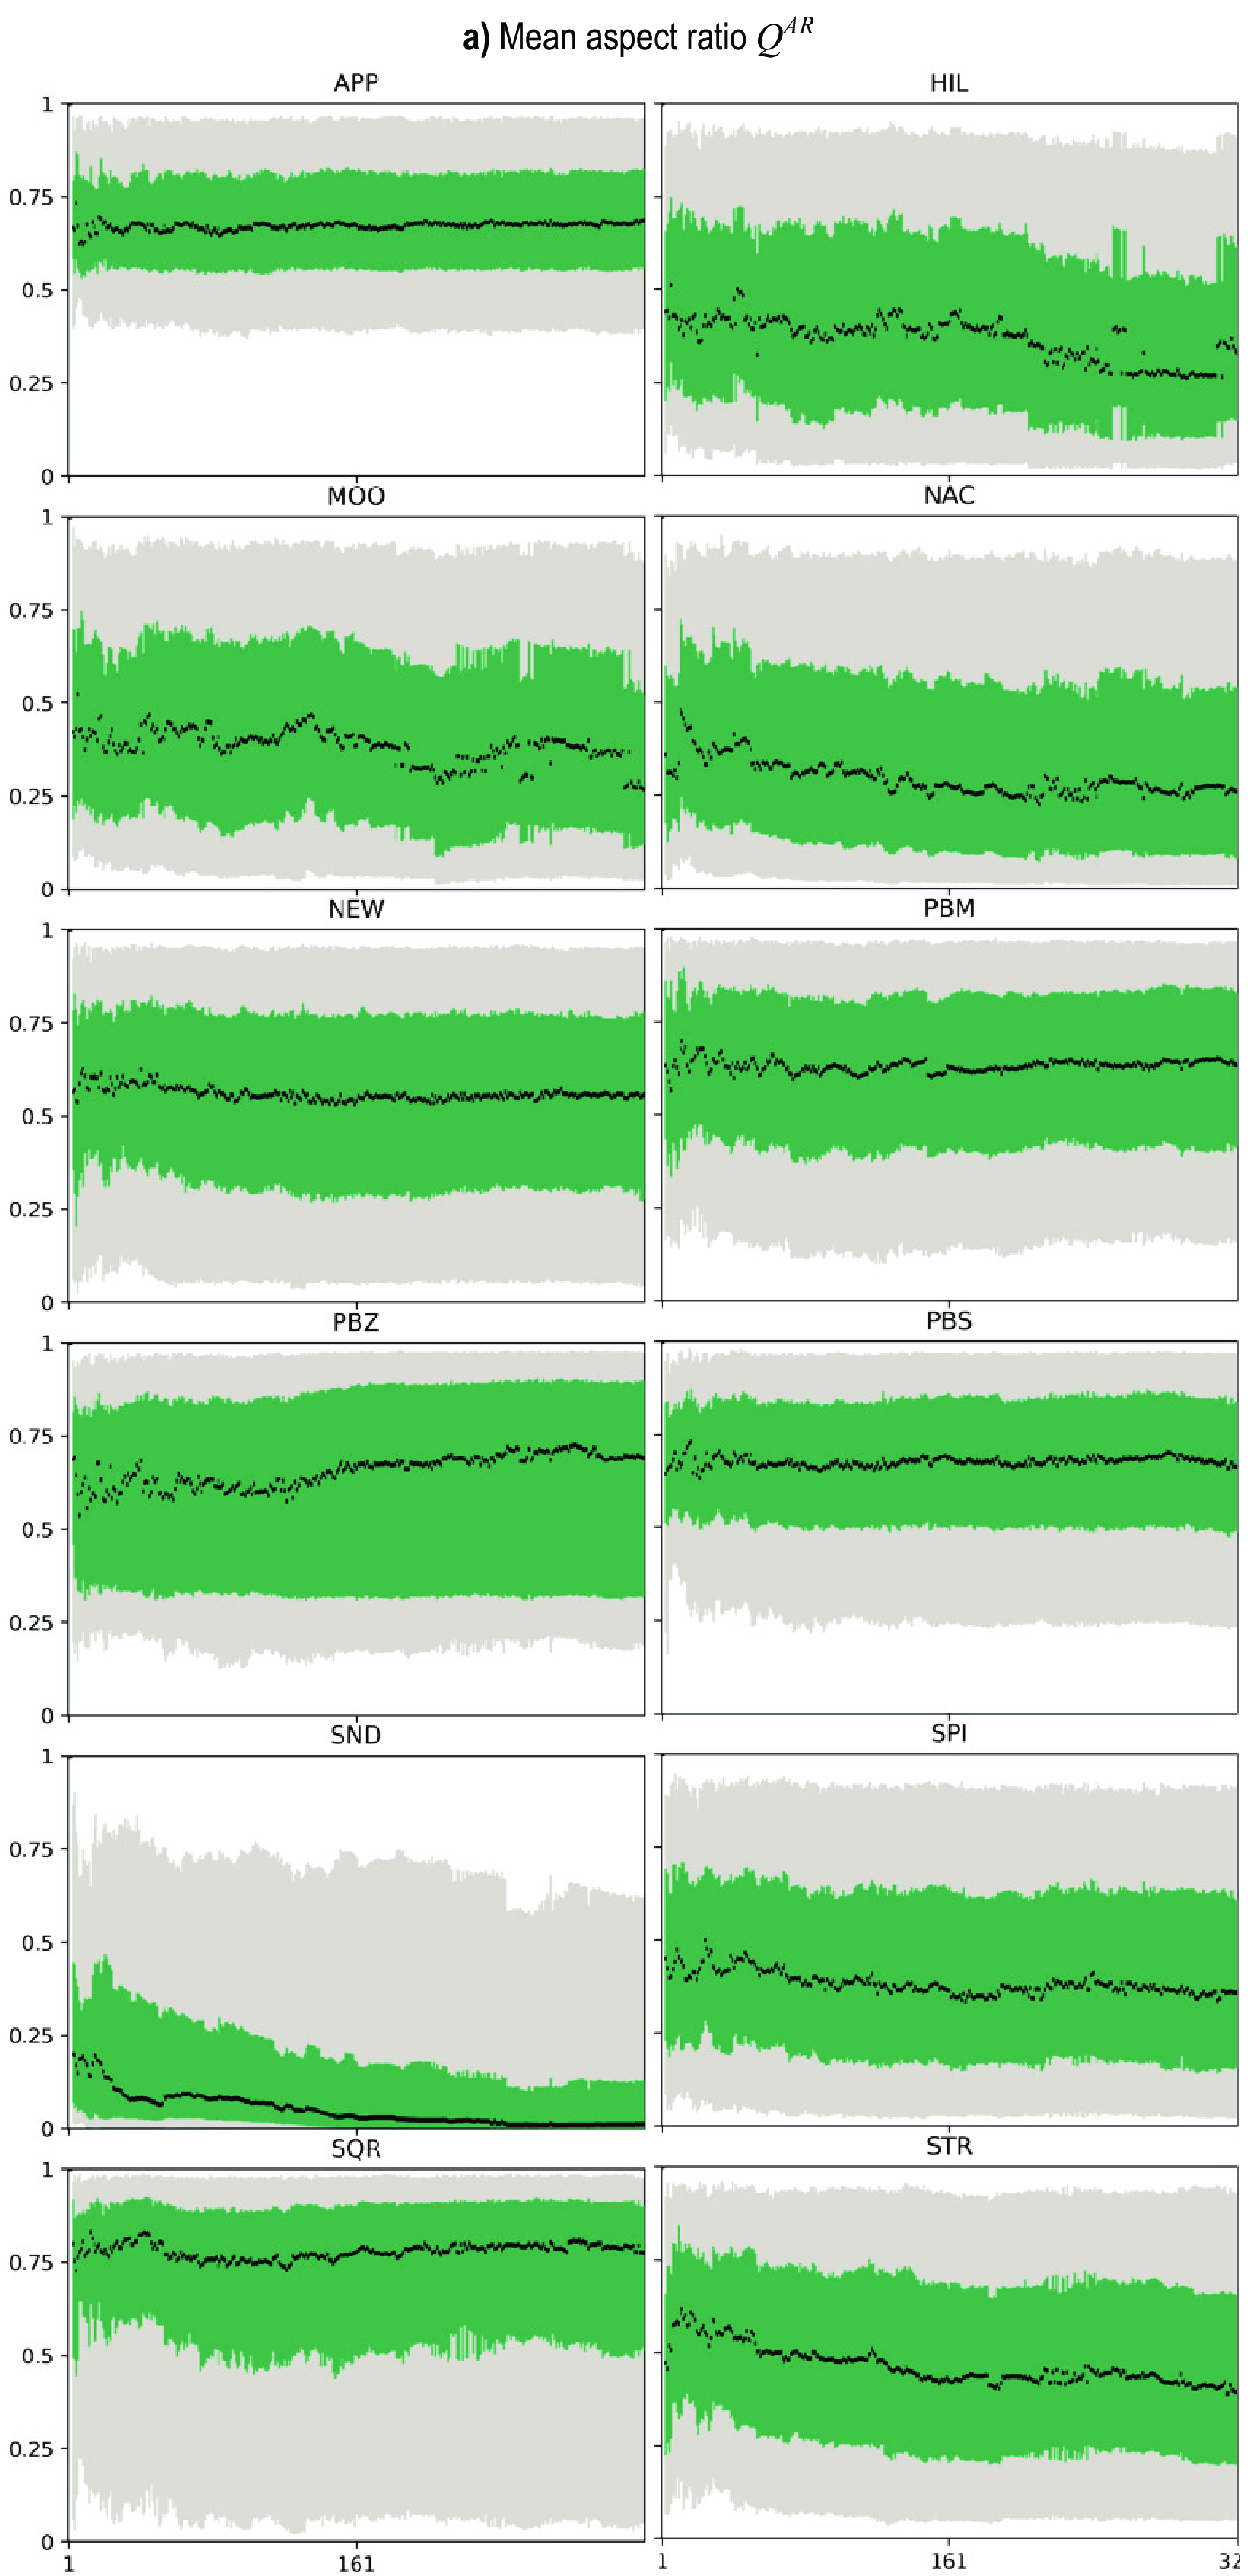
\includegraphics[width=.8\textwidth]{figures/initial-treemap-evaluation/boxplot-a.png}
%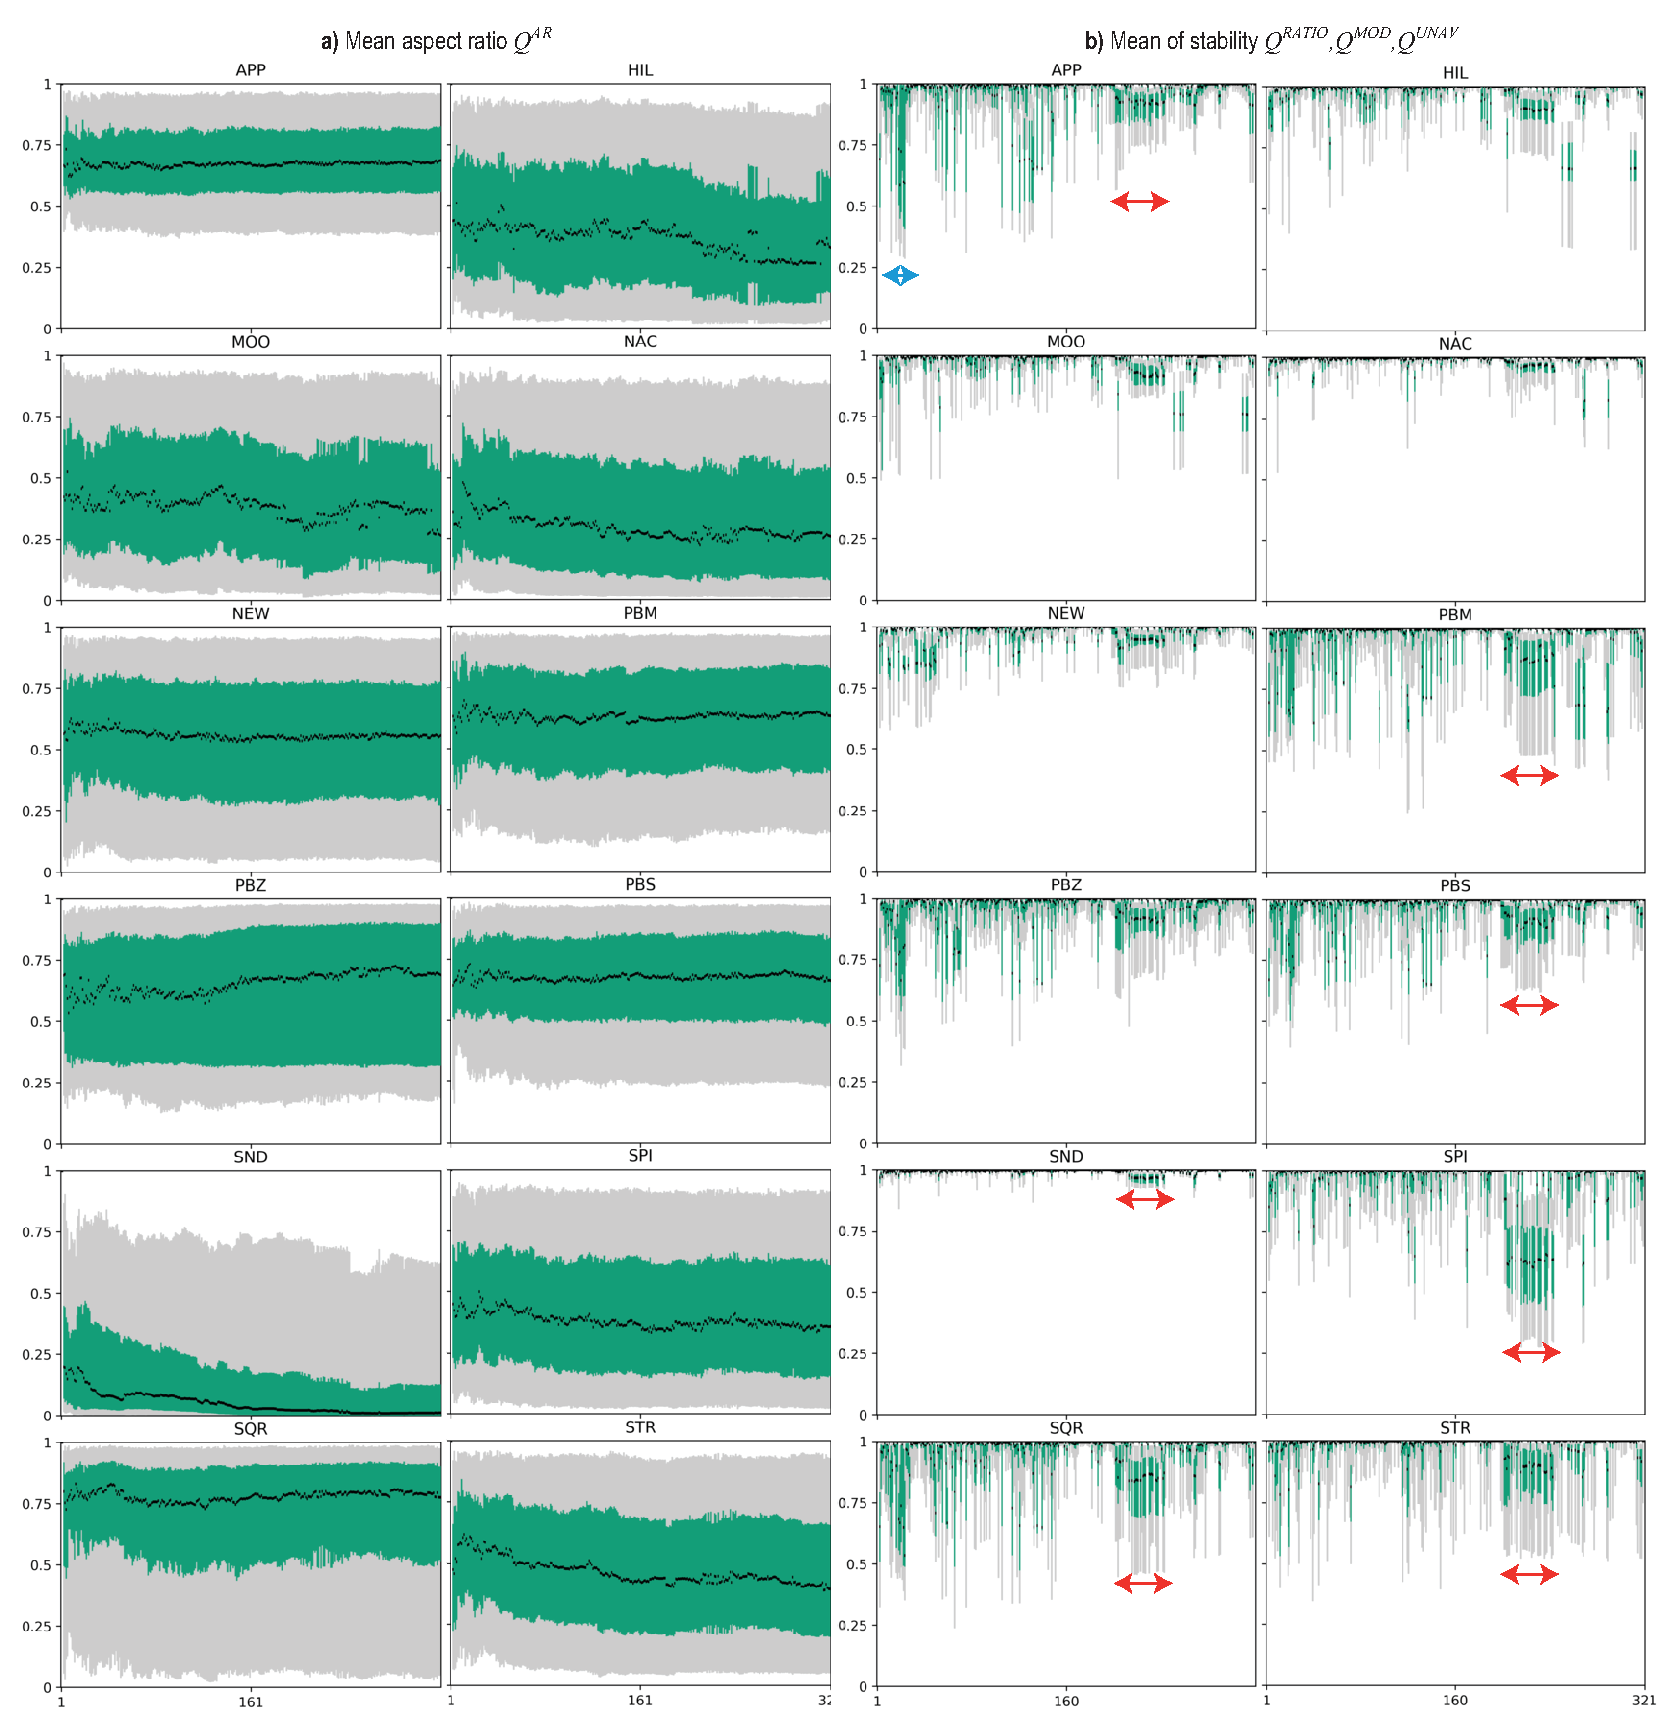
\includegraphics[width=1.0\linewidth]{figures/boxplots.eps}
\vspace{-0.25cm}
\caption{Evolution in time of spatial quality for the \emph{cpython} dataset.}
\label{fig:boxplots_1a}
\end{figure*}

\begin{figure*}[htbp!]
\centering
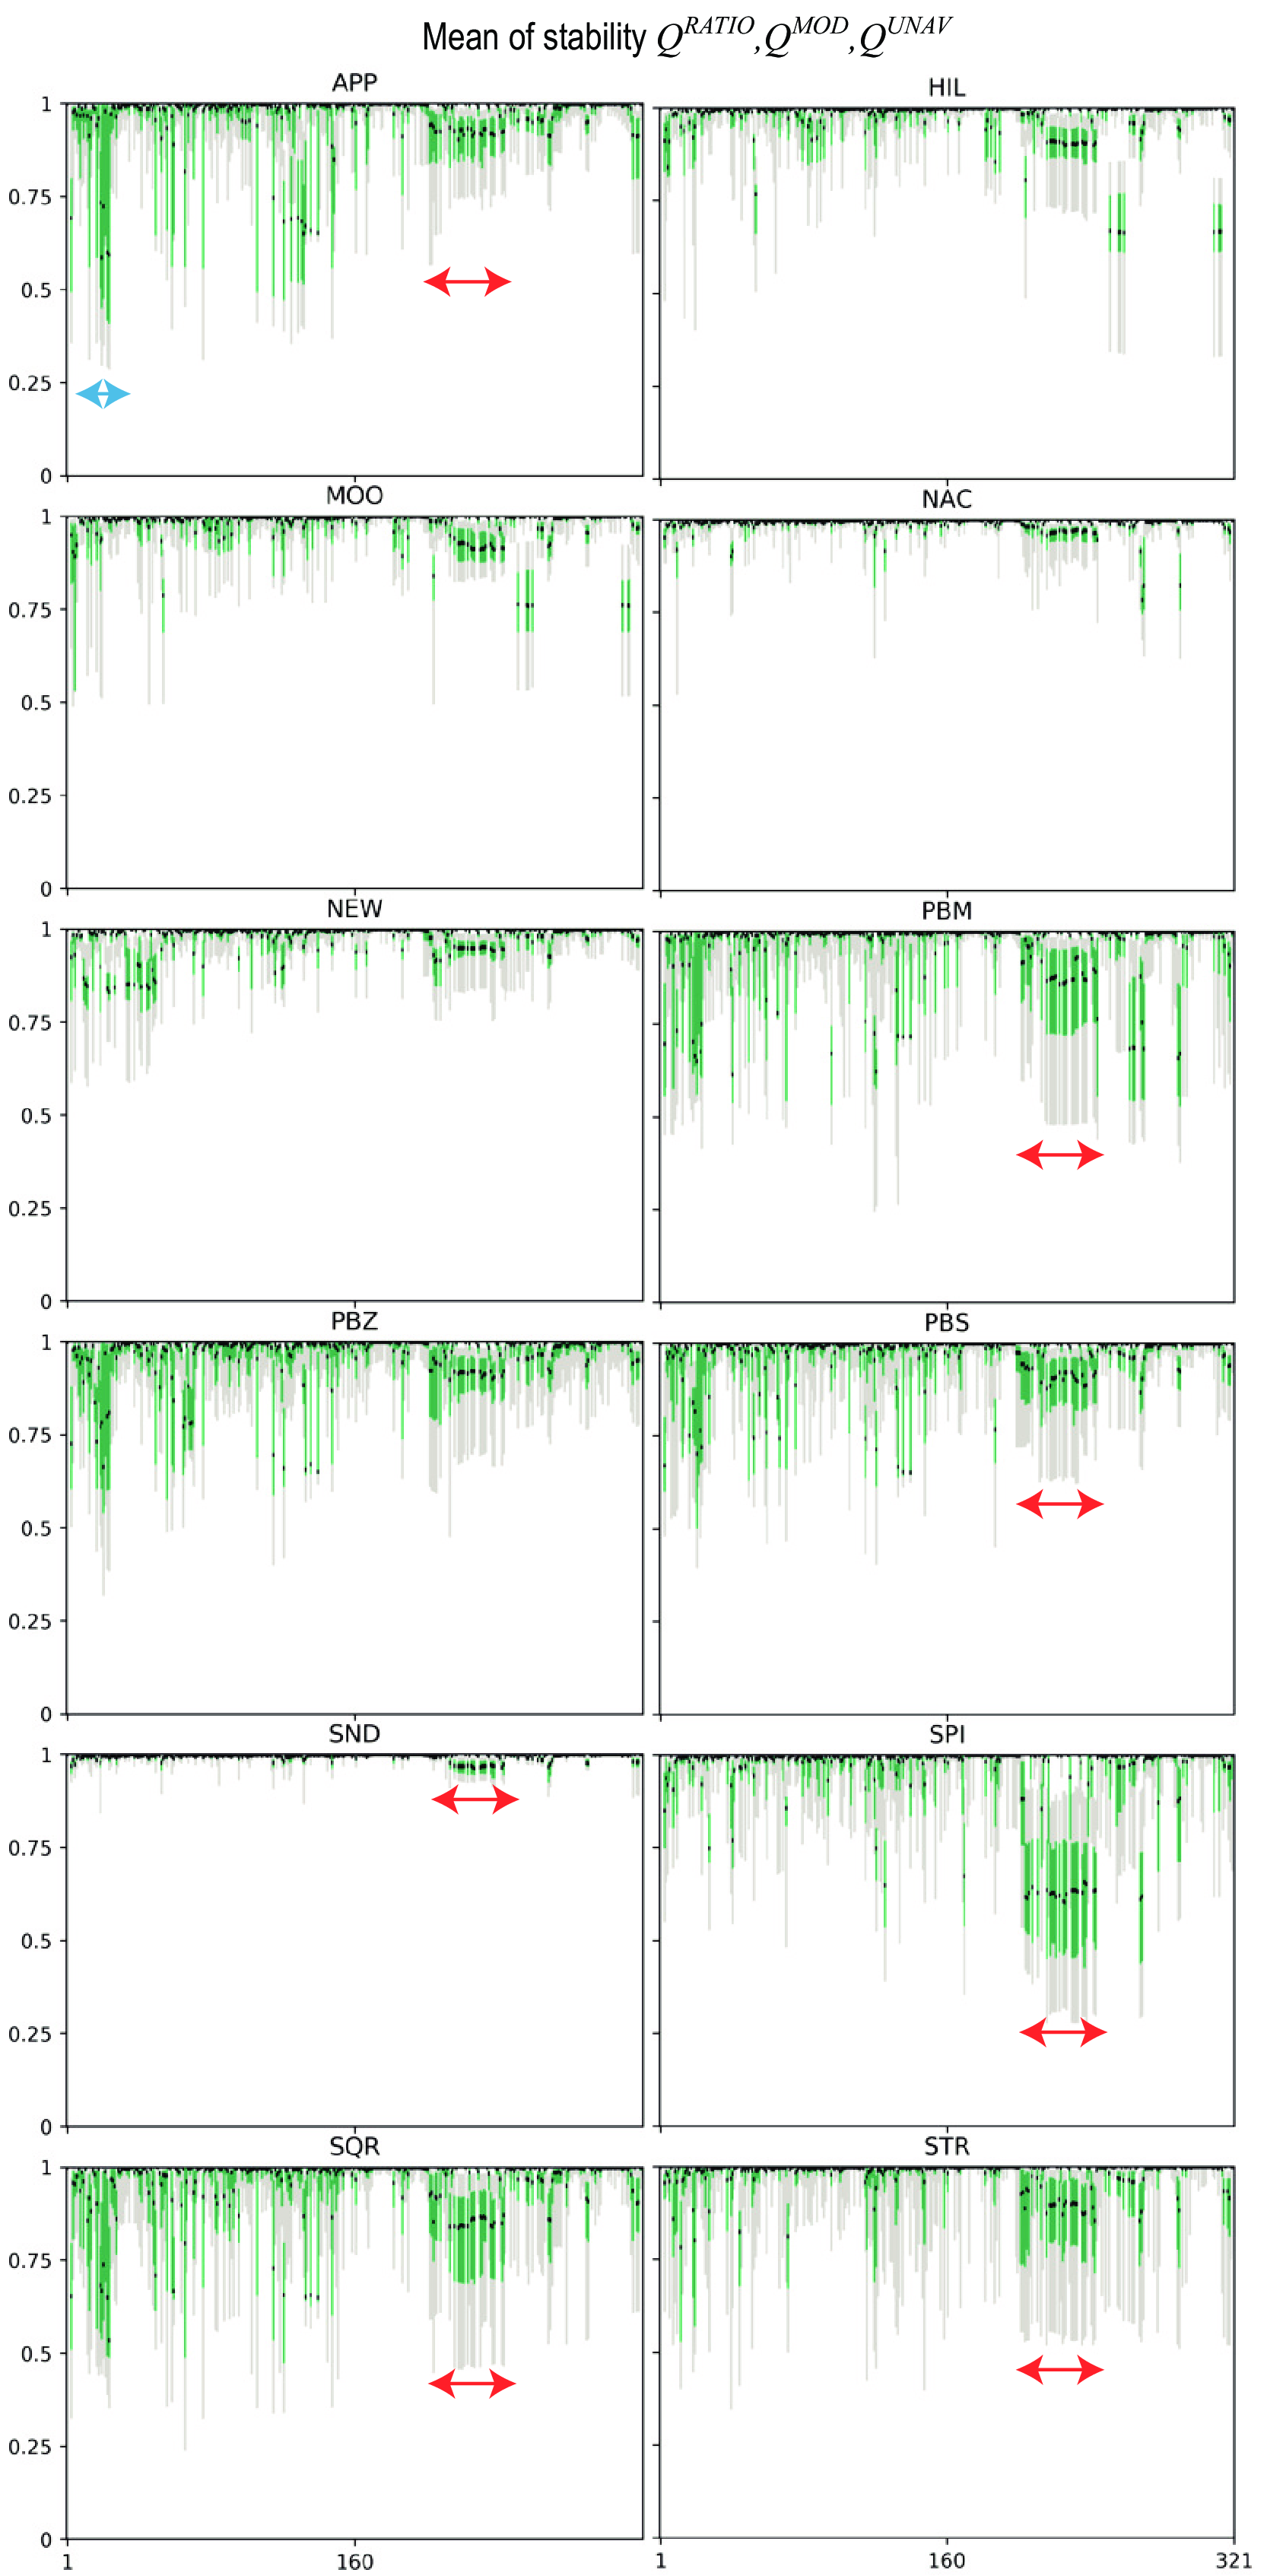
\includegraphics[width=.8\textwidth]{figures/initial-treemap-evaluation/boxplot-b.png}
%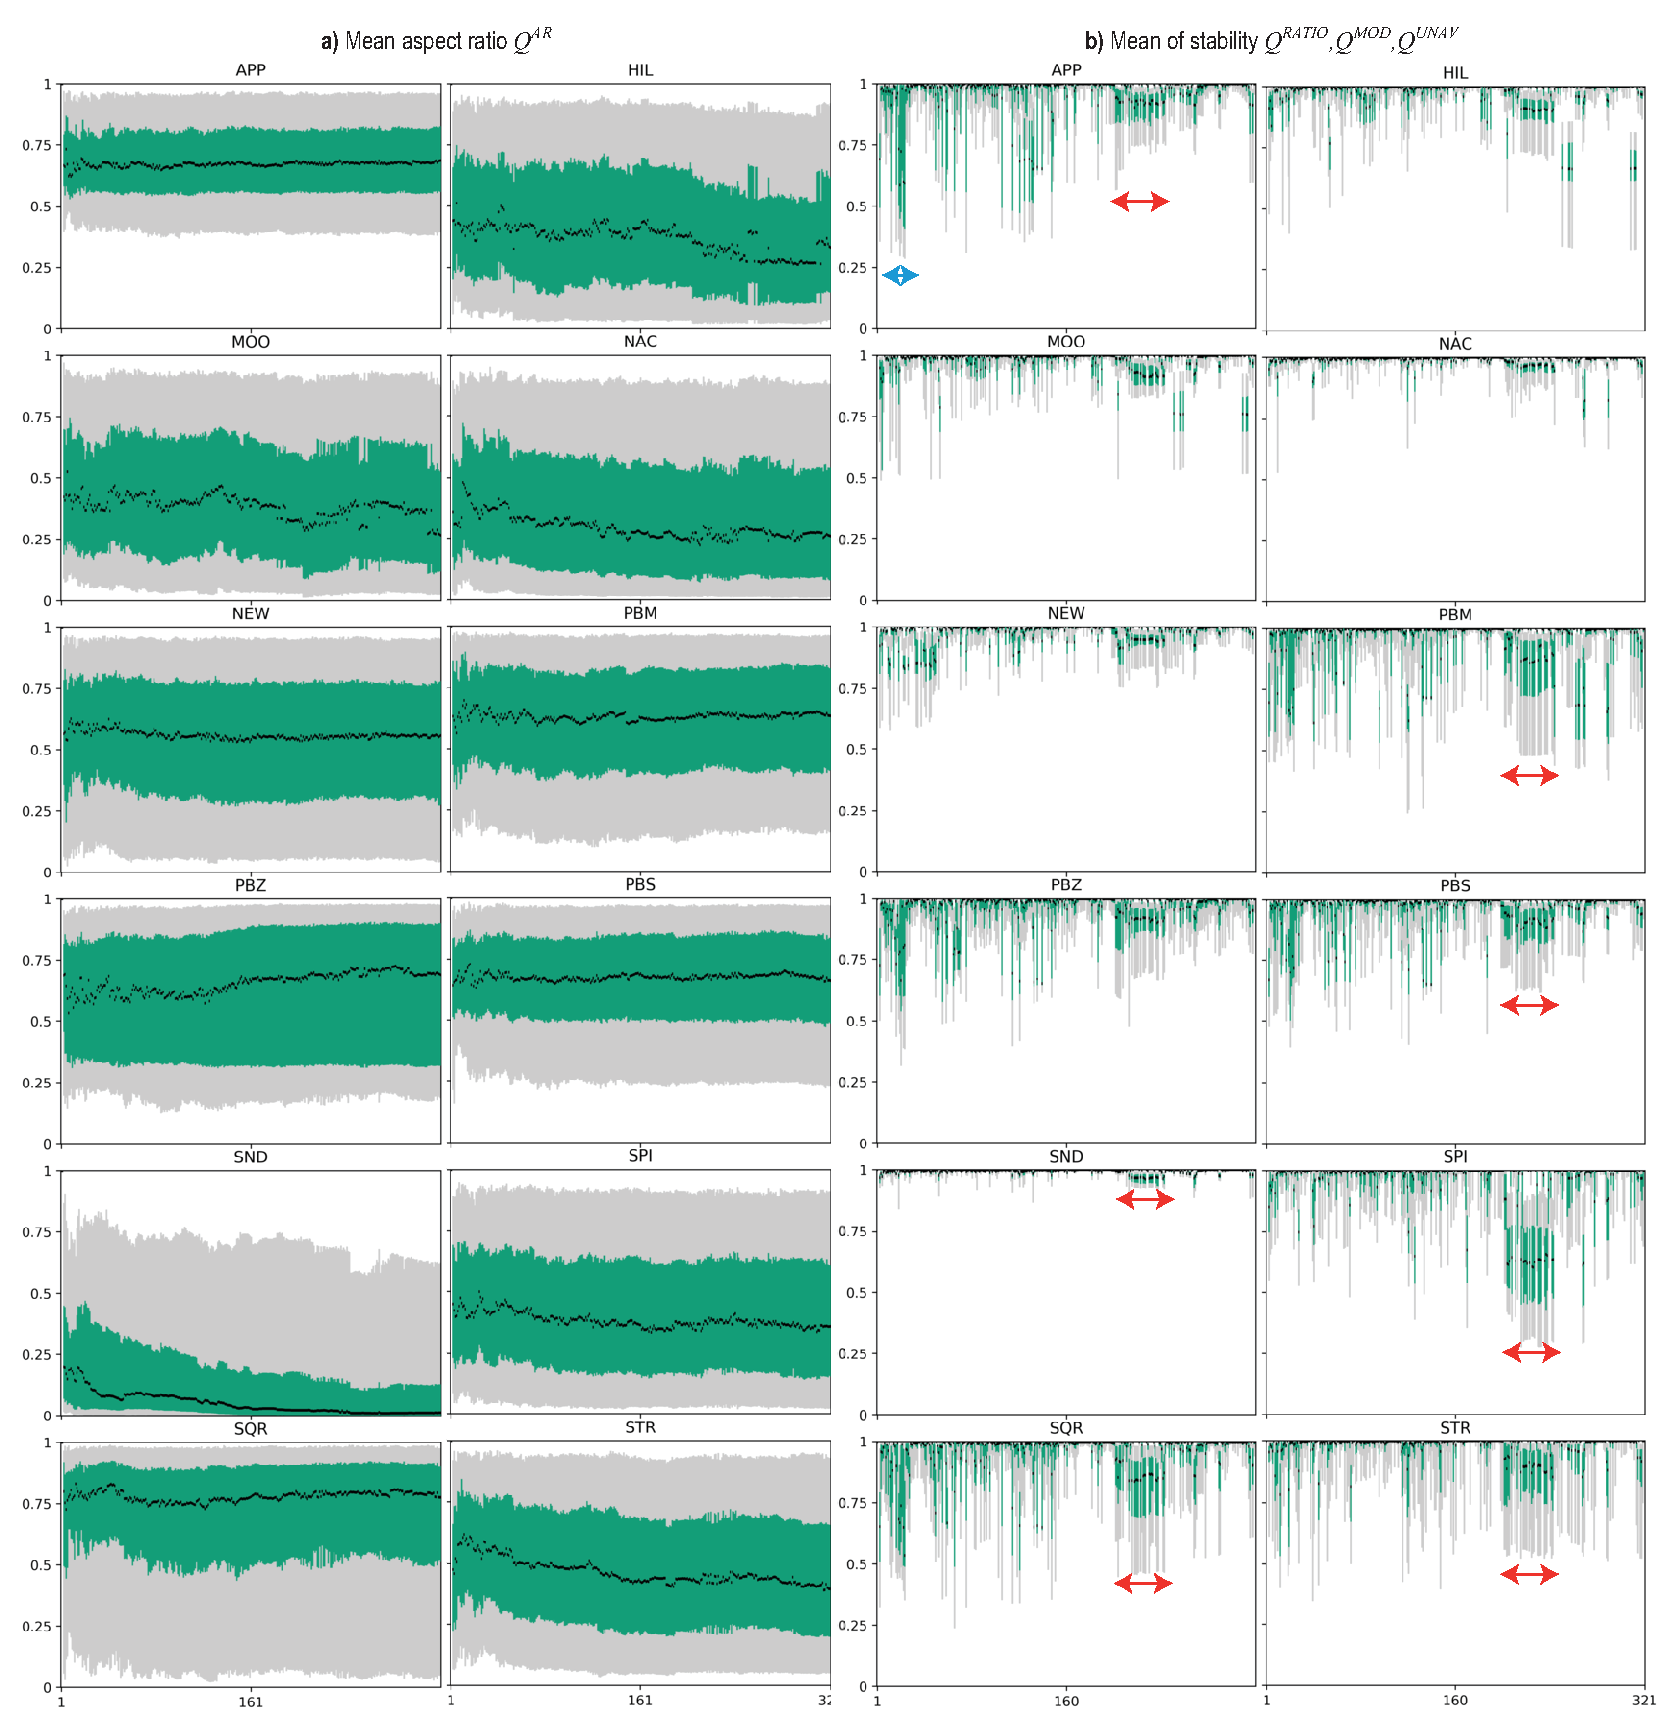
\includegraphics[width=1.0\linewidth]{figures/boxplots.eps}
\vspace{-0.25cm}
\caption{Evolution in time of the averaged four stability metrics for the \emph{cpython} dataset.}
\label{fig:boxplots_1b}
\end{figure*}

Figure~\ref{fig:boxplots_1a}a shows the evolution of the $Q^{AR}$ metric (Eqn.~\ref{eqn:spatial_ratio}) for all tested methods for \emph{cpython}. We see that APP and PBS deliver overall quite high and constant-over-time aspect ratios (0.7), so they are the best methods for spatial quality, with APP being better as it has a narrower $Q^{AR}$ spread around a slightly higher median value. SQR scores higher median values, but has a larger spread -- for every revision, it can score as bad as 0.05 aspect-ratio, while APP does not drop below 0.4 (compare the bottoms of the gray bands in Fig.~\ref{fig:boxplots_1a} for APP and SQR). SND shows the worst spatial quality, with a tight spread around a median $Q^{AR}$ below 0.1. The chart also tells us that most methods deliver \emph{consistent} spatial quality regardless of the data changes in the 321 revisions (which we found to be large by manually examining the sequence). The quality decrease shown by SND and (less) by HIL and STR is somehow surprising, as none of the studied methods uses a `history' of the tree-sequence in its layout heuristics.

Figure~\ref{fig:boxplots_1b}b shows the evolution of four stability metrics $Q^{RATIO}$, $Q^{MOD}$, and $Q^{UNAV}$, averaged per time-step. Compared to spatial quality, we see now much more variation between methods and also much more variation (of the stability) over time. We see that SND is by far the most stable method, whereas SQR, SPI, and PBM score worst. Long `icicle' like boxplots indicate revisions where much more visual change was present than `warranted' by the data change. Interestingly, these appear at the same moments for different algorithms (Fig.~\ref{fig:boxplots_1b}b, red markers shows one example). For such moments we see large variations across methods: For SPI, this is the most unstable part of the sequence, both in median and 5-95\% range sense, whereas APP finds earlier sequences (marked in blue in Fig.~\ref{fig:boxplots_1b}) which are harder to lay out stably.

%
% Refinements:\\
%
% Aggregate all the metrics in the same family (AR and STAB) when you generate every single plot (so, for one dataset, we will have M*2 plots, two plots (AR and STAB) for every of the M methods).
% We also cannot have 30*M*2 plots in the paper. So, select 1..max 2 interesting datasets, like, the largest ones, to generate these plots (so we have in total either 2*M or 4*M individual plots).
% make sure, when you generate the plots, that you use the most up-to-date definitions of AR and STAB metrics! We used some pretty old/early versions of these in the snapshot above.


\subsection{How do methods perform on different datasets (Q3)?}
\label{sec:q3}
%
%
So far, we presented charts that aggregate over all datasets (Sec.~\ref{sec:q1}) or focus on a single dataset, but aggregate all stability metrics (Sec.~\ref{sec:q2}). We would like to see how the proposed stability metrics compare to each other, as we are still in the process of understanding their measurement characteristics. Also, we would like to see how these metrics vary over several datasets. For these goals, we use a set of table views, one per quality metric. In each table, columns are datasets and rows are algorithms. Each cell thus encodes the average value of one quality metric for one dataset tested by one algorithm. Cells are colored with a luminance-based colormap, with data values separately normalized per metric table, so that darkest cells indicate worst cases in all tables (but with potentially different metric absolute values), and brightest cells indicate best cases in all tables.

\begin{figure}[htbp!]
\centering
  \includegraphics[width=.8\linewidth]{figures/initial-treemap-evaluation/matrixplots.eps}
\vspace{-0.1cm}
    \caption{The five quality metrics for all tested methods, all datasets.}
\vspace{-0.2cm}
  \label{fig:table}
\end{figure}

Figure~\ref{fig:table} tells several interesting things. Scanning the first table row-wise, we see that there are no large aspect-ratio quality differences between the tested datasets. This says that most methods (with the notable exception of SND) achieve quite good aspect ratios for a wide dataset variation. Over all datasets, APP is the best method, surpassed by SQR only for a few datasets. Conversely, we see that SND is the most stable method with respect to all four considered stability metrics. Stability-wise, we see that some datasets (\emph{hospitalrun-frontend}, \emph{Leaflet}, and \emph{PhysicsJS}) consistently score worse than all others for basically all algorithms. These are also the datasets yielding the worst stabilities, when PBM, SQR, STR, and SPI methods are used. This indicates that these methods are quite sensitive in stability on the type of input dataset so, for obtaining higher stabilities, other methods should be used. At a higher level, we see that the $Q^{RATIO}$, $Q^{MOD}$, and $Q^{UNAV}$ stability metrics yield very similar plots. This is an interesting finding, since the metrics have quite different formulations (Sec.~\ref{sec:init_metrics}), and indicates that the results can be trusted -- the chance of three metrics having such different expressions yielding so similar values being very small. In contrast, the $Q^{CORR}$ metric has much lower values, which is explained by the fact it is much more conservative -- a good algorithm would need to yield very well correlated $\delta a_k$ and $\delta c_k$ values, and we have seen in Sec.~\ref{sec:q1} that this is by far not the case. We conclude that visual \emph{vs} data change correlation is a too strong quality desiderate for dynamic treemaps handing large real-world datasets, and advise next to use in practice any of the $Q^{RATIO}$, $Q^{MOD}$, and $Q^{UNAV}$ metrics to gauge stability, or, as we have done in Sec.~\ref{sec:q3}, their average value.

\begin{figure*}[htbp!]
\centering
%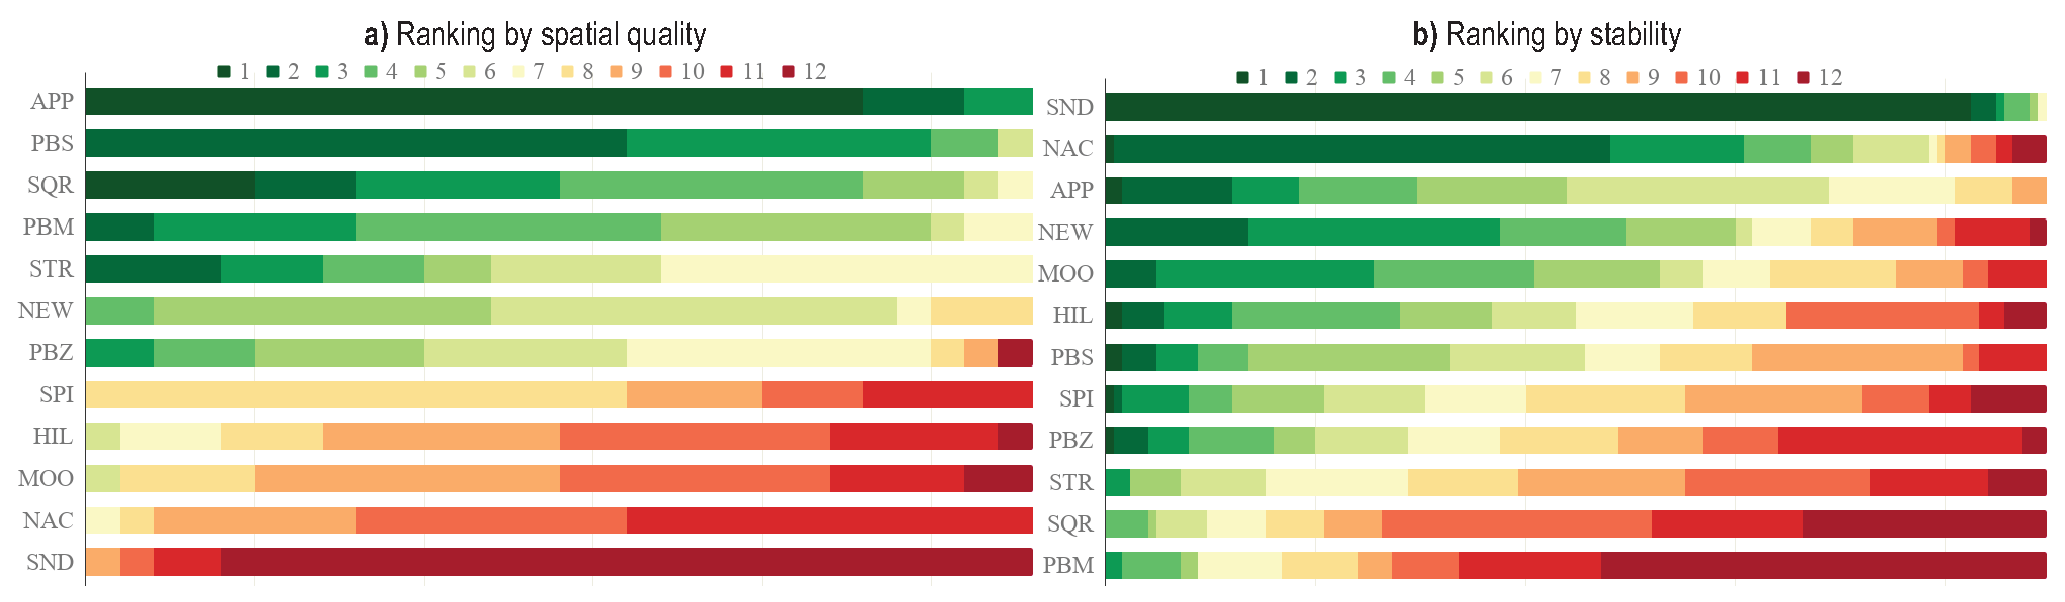
\includegraphics[width=.8\textwidth]{figures/rankcharts.eps}
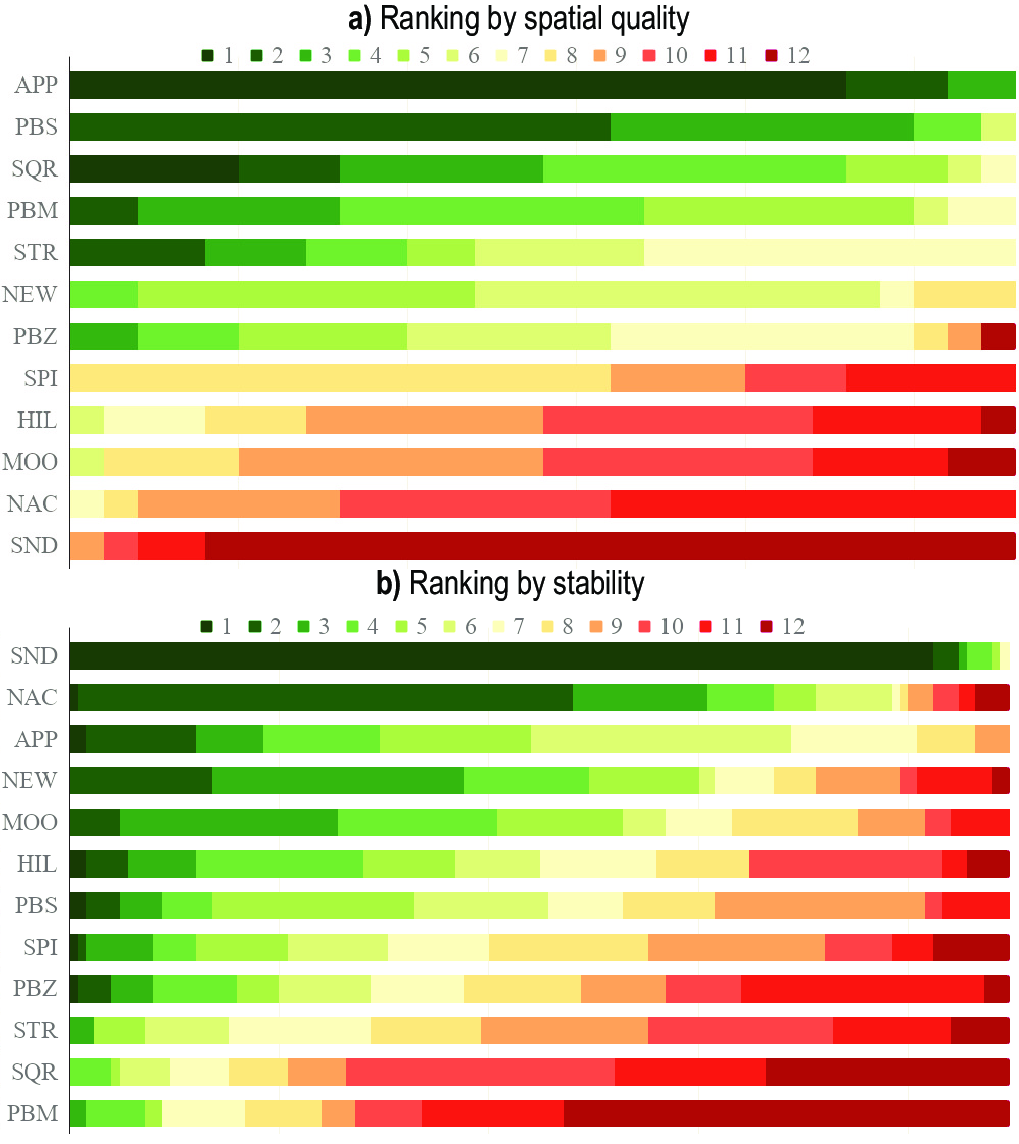
\includegraphics[width=0.9\textwidth]{figures/initial-treemap-evaluation/rank-vertical.png}
\vspace{-0.1cm}
\caption{Ranking of the 12 methods showing the percentage of times they scored a certain rank with respect to spatial quality (a) and averaged stability (b).}
\vspace{-0.2cm}
\label{fig:rankchart}
\end{figure*}

\subsection{How to summarize the comparison (Q4)?}
\label{sec:q4}
%
%
The visualizations so far (Q1--Q3) have given us several insights: We have seen that APP, PBS, and SQR are the best methods with respect to spatial quality, while SND performs poorly for that, but it is the best for stability; different methods have quite different spreads of quality over a given tree sequence, some delivering more consistent results than others, but for most algorithms do not degrade over time; and several of the proposed stability metrics are strongly correlated. It is now useful to \emph{summarize} our findings to present a compact ranking of the tested methods. For this, we use two stacked bar charts. Each bar maps one method and is divided into segments. A segment's length tells the percent of the total number of versions (of all datasets) for which that method had a specific rank regarding spatial quality (Fig.~\ref{fig:rankchart}a) and averaged stability metrics (Fig.~\ref{fig:rankchart}b). We color segments by an ordinal colormap to show these ranks (1 being the best and 12 being the worst). Bars (methods) are sorted in each chart to put the one with highest average rank, weighted by the percents of the total number of versions for all obtained ranks, at the top (Fig.~\ref{fig:rankchart}). From Fig.~\ref{fig:rankchart}, we first see that spatial quality and stability are strongly inversely correlated -- methods that score well on one tend to score poorly on the other. We also see that the top methods in both charts are very good for \emph{most} of the tested datasets, \emph{i.e.}, it is easy to find a method that optimizes either spatial quality or stability, but not both. Interestingly, APP (a less known method) is better in spatial quality, and significantly better in stability, than SQR (arguably the method of choice for creating good aspect-ratio treemaps), so it should be preferred to SQR. Similarly, for stability, APP and NEW (two less known methods) are in the top-four most stable methods, and while worse than SND (very well known method), they have higher spatial quality, so they should be preferred to SND.

\begin{figure}[htbp!]
\centering
%\includegraphics[width=.4\textwidth]{figures/starplot.eps}
\includegraphics[width=.85\linewidth]{figures/initial-treemap-evaluation/starplot.eps}
\vspace{-0.1cm}
\caption{Summarized comparison of all methods (colored dots) on all datasets (colored lines) \emph{vs} spatial quality and stability.}
\vspace{-0.2cm}
\label{fig:starplot}
\end{figure}

A disadvantage of the rank charts in Fig.~\ref{fig:rankchart} is that they do not easily allow linking spatial quality and stability. To alleviate this, we propose a final visualization which uses a start plot metaphor (Fig.~\ref{fig:starplot}). The scatterplot points (circles, categorically colored) are methods attributed by their average spatial quality and stability over all datasets, all revisions. Each method is linked with the 28 tested datasets by same-color lines; a line's endpoint has the average spatial quality and stability over all its revisions for the corresponding method. The plot conveys several insights: First, methods follow roughly a concave curve (Fig.~\ref{fig:starplot}, thick dashed curve), telling the trade-off between spatial quality and stability. Variation in average spatial quality is much larger (roughly 45\%) than in average stability (roughly 8\%). The fan-out of lines from a method shows how predictable that method is, and here we see large variation over methods, with \emph{e.g.} APP being quite consistent in spatial quality, while MOO, STR, and SND show large dataset-dependent variations in both spatial quality and stability (see Fig.~\ref{fig:starplot}, thin dashed curves). The latter is especially interesting: Even though SND has the highest average stability, it can also score worse than many other methods on certain datasets.

To conclude, it is hard to designate an `optimal' method, as this strongly depends on which of stability and spatial quality users see as most important for their concrete use-cases, and by how much. Still, based on all our insights, we believe that APP offers a very good compromise -- very high spatial quality and overall stability similar to most methods, surpassed only (and not in all cases) by SND.


\section{Discussion}
\label{sec:init-discussion}
%
%
Let us discuss our results in the light of the dimensions of evaluating treemap algorithms for software evolution visualization (Sec.~\ref{sec:current_state}):\\

\noindent\textbf{Algorithms:} We consider 12 well-known treemap methods, in contrast to typically 2--3 techniques in current treemap evaluations in software visualization papers. We argue that this gives valuable insights on the suitability of such well-known methods for handling evolving software trees, so it makes the choice of a given method easier for the software visualization practitioner. For instance, our evaluation can tell the interested user which are the advantages (or limitations) of a \emph{given} algorithm \emph{vs} another given algorithm, from the perspectives of spatial quality or stability.\\

\noindent\textbf{Datasets:} Our treemap benchmark cannot cover all variations of trees extracted from software evolution use-cases. However, it measures in total roughly $1.9 \cdot 10^{9}$ treemap cells for 28 tree sequences up to 321 time-steps (revisions). The size and variability of tree sequences covered by our study is larger than all existing similar evaluations of dynamic treemaps in software visualization. However, we admit that we cannot \emph{extrapolate} from this evaluation to draw statistically strong conclusions concerning the quality of a given treemap algorithm for the \emph{entire} space of evolving software hierarchies. Doing so would require (a) a characterization of this space in terms of objective metrics (\emph{e.g.}, tree size, depth, type of structure, type of changes); (b) a targeted search of software repositories to extract trees which `sample' well all these dimensions; (c) an evaluation of our metrics on this benchmark; and (d) most importantly, finding possible correlations between the measured performance of algorithms and the characteristics of the tree sequences they work on. We acknowledge these limitations, and outline them as important directions for future work.\\

\noindent\textbf{Metrics:} We measure treemap stability by essentially considering the first derivative of the treemap algorithm function mapping from tree-node weights to rectangular cell-sets. We detail four variants for measuring stability this way, and observe that three of them, while quite different in terms of actual definitions, yield very similar results. We believe this is an important finding, as it motivates the idea of defining stability by relating visual change to data change. The fourth stability metric (Pearson correlation) showed however to be of limited practical use, as typical dynamic treemaps exhibit a too low correlation of the data and visual changes as compared to other phenomena where this metric is used. This can also indicate that dynamic treemaps may exhibit a more \emph{complex} form of data \emph{vs} visual change correlation than a \emph{linear} one. 
Concluding, we argue that measuring stability by involving both visual and data change is desirable, but we acknowledge that more work is needed to further refine the definition of the proposed stability metric, so that it avoids potential normalization biases, and it also captures in a more demonstrable way what actual users perceive as `unstable'.\\

\noindent\textbf{Result exploration:} We present five visualizations of treemap quality metrics, covering all involved dimensions: cells, revisions, datasets, metrics, and algorithms. As the dimensionality of this data space is large, we obviously cannot cover \emph{all} possible viewpoints. Yet, our visualizations help finding novel insights on the behavior of dynamic treemaps for evolving software hierarchies, and also confirm earlier observations, \emph{e.g.} the known stability of SND. Our visualizations can be used to both analyze fine-grained details (at cell level) and present aggregated conclusions (at algorithm level). They can help the practitioner in understanding what is gained, and/or lost, by choosing a certain treemap algorithm instead of another one.\\

\noindent\textbf{Replicability:} All our results (datasets, treemap and visualization code, measurements) are available online at~\citep{benchmark}. To our knowledge, this is the first benchmark for (dynamic) treemaps for applications in software evolution understanding. It can serve both for practitioners interested in choosing an algorithm based on specific quality criteria, but also for researchers aiming to benchmark their new algorithms, with limited effort, against existing ones.\\

\noindent\textbf{Limitations:} There are several points which can be covered better. First and foremost, as mentioned, we need a more principled sampling of the space of trees extracted from software evolution to gain more confidence in the obtained quality results (or how these would differ as a function of the tree sequences' characteristics). We argue that our current work, \emph{i.e.} the \emph{automated} set-up of the extraction pipeline of dynamic trees from software repositories, computation of the proposed quality metrics, and visualizations that aggregate these, forms the necessary basis for such extensions, which we consider as future work. Separately, more treemap algorithms could be considered, \emph{e.g.}, Voronoi, hybrid, or bubble ones. This will require an adaptation of the spatial quality and stability metrics so they can be used for non-rectangular cells.\\

\noindent\textbf{Threats to validity:} Similar to software quality, we measure treemap quality by a number of `proxy' metrics. While we argue for these metrics at technical level (see the stability metric \emph{vs} function continuity discussion) or, separately, reuse well-known metrics (see the aspect-ratio metric), we do not have hard evidence that such metrics truly capture quality as seen by the eyes of the beholder (end user). The advantage of using such `intrinsic' quality metrics is that they can be computed automatically, on a large benchmark, and are independent on actual tasks, users, or use-cases. This allows for direct and objective comparisons, parallel to what is done on the context of \emph{e.g.}  Graph Drawing \citep{hachul,battista}, where metrics such as number of crossings, angle of crossings, and distribution of edge lengths are used to rank the quality of graph drawing algorithms. 
The disadvantage is that we cannot directly infer, from such metrics, how fit to purpose a given treemap technique will be given a specific user, use-case, type of dataset, and task. We argue for our approach as follows: \emph{if} for a given user, use-case, and task, one agrees that a good treemap algorithm should have the properties captured by our quality metrics, \emph{then} one can use our evaluation and related artifacts (benchmark, metrics, visualizations) to find the best suitable algorithms.


\section{Conclusions}
\label{sec:conclusions}
%
We have presented an evaluation of treemap algorithms for the visualizaton of dynamic tree sequences extracted from the evolution of software repositories. For this, we proposed a benchmark formed by 28 datasets extracted from well-known software repositories, five metrics that aim to capture spatial quality and stability, and 12 known treemap methods. We also propose six visualizations aimed at interpreting the measurement results from several angles, covered by four types of questions. All results (datasets, treemap implementations, measurement code, and visualizations) are publicly available and can constitute the basis of a benchmark for treemap evaluation for visualizing evolving software hierarchies. 

Several directions exist for extending this work. First and foremost, a finer-grained analysis of the space of evolving software trees can be made to elicit correlations between characteristics of the datasets and measured quality of the tested treemap methods. Secondly, and at a higher level, it would be useful to extend this type of benchmarking to other application domains that generate dynamic trees and use treemap methods to visualize their evolution in time. This second direction of work will be further explored in the next chapter.

